\chapter{Системийн шинжилгээ}
\section{Шаардлагууд}
\subsection{Хэрэглэгчийн шаардлага}

\begin{itemize}
  \item Хэрэглэгчийн алгоритм ба програмчлалын мэдлэгийг бататгаж, цааш өөр бодлогуудаар сорьдог байна.
  \item Хэрэглэгчид загвар код харуулж, бодох процессийг илүү хялбарчилсан байна.
  \item Програмчлалын үндсэн ойлголттой ямар ч хэрэглэгчид аппликейшн нь хэрэглэхэд ойлгомжтой, хүртээмжтэй интерфейстэй байна.
  \item  Хэрэглэгч өөрт тохирох дизайныг сонгож, customize хийх боломжтой байна.
  \item Хэрэглэгчид зориулсан editor нь хэрэглэгчийг бичиж байх үйл явцыг сонсон хурдан хариу өгөх intellisense-тэй байна.
  \item Хэрэглэгч амжилттай бодлогоо бодсоноор бусдын кодын хэрэгжүүлэлт, шийдлүүдийг харах боломжтой байна.
  \item Програмчлалын Python, Javascript болон C/C++(\textit{optional}), JAVA(\textit{optional}) хэлнүүд дээр бодлогыг бодох боломжтой байх.
  \item Хэрэглэгч кодоо ажиллуулах үед тэнцсэн эсвэл тэнцээгүй эсэхийг нь хэрэглэгчид мэдэгддэг байх ёстой.
  \item Систем нь монгол хэл бүхий хэрэглэгчийн интерфейстэй байх ёстой.
\end{itemize}

\subsection{Системийн шаардлага}
\begin{itemize}
  \item Сервер лүү brute-force байдлаар халдалт хийхээс сэргийлсэн байх.
  \item Өгөгдлийн сан руу хэрэглэгчид зөвхөн сервисүүдээр дамжин хандалт хийж болдог байх.
  \item Систем нь 24/7 ажиллагаатай байх бөгөөд хэзээ ч, хаанаас ч хандах боломжтой байна.
  \item  Бодлогын сан нь дахин сэргээх боломжтойгоор гараар backup хийдэг байна.
  \item Ачаалал даах чадвартай байх бөгөөд ямар нэгэн ачааллаас үүдэлтэй асуудал гарвал унтралгүйгээр тодорхой хугацааны дараа хэвийн ажиллагааг хангадаг байх.
  \item Хэрэглэгчээс оруулсан сэжиг бүхий кодууд compiler сервер дээр ажилладаггүй байна.
  \item Бодлого бүр тест кэйстэй байх шаардлагатай.
  \item Систем нь хэрэглэгчийн мэдээлэл болон бодсон бодлогуудын мэдээллийг хадгалдаг байх ёстой.
  \item Хэрэглэгчээс орж ирэх кодыг гуравдагч систем рүү хандах боломжгүй орчинд ажиллуулж үр дүнг гаргадаг байх хэрэгтэй.
\end{itemize}

\clearpage

\section{Технологийн асуудлууд}
"Coldbrains" систем нь програмчлалын бүтээгдэхүүн дотор програмчлалын үйл явцыг явуулж байгаа тул юун түрүүнд аюулгүй үйл ажиллагаа болон найдвартай байдлыг хангадах байх хэрэгтэй билээ. Нээлттэй вебсайтаар дамжуулан гадны ямар ч хэрэглэгч хэрэглэх боломжтой бөгөөд зохисгүй хэрэглэгчдийн үйл ажиллагааг хязгаарлах маш олон програмчлалын асуудлууд бий болж байна.

\subsection{Middleware}
Кодыг хүлээн авч ажиллуулж буй серверийг хэрэглэгчээс хязгаарлахын тулд тухайн хэрэглэгчийн веб аппликейшн болон серверийн хооронд middleware сервер байх бөгөөд энэхүү сервер нь хэрэглэгчээс ирэх хүсэлтүүдийг боловсруулан цааш дамжуулдаг байх шаардлагатай билээ. Үүнд:
\begin{itemize}
  \item Хэрэглэгчээс богино хугацаанд ирэх олон хүсэлтүүдийг хязгаарлах
  \item Жинхэнэ серверийн IP хаягийг нууцлан улмаар зөвхөн өөр дээрээсээ дамжуулах
  \item Хэрэглэгчийн эрхийг(user credentials/access token) шалгах
  \item Frontend-ээс ирэх Payload-ийг encrypt хийх
\end{itemize}
зэрэг үүргүүдийг гүйцэтгэх билээ.

\subsection{Sandboxing}
Middleware-ээр дамжуулагдан ирсэн кодыг аюулгүй эсвэл хортой код гэдгийг ялгах боломжгүй учраас тухайн кодны ажиллах орчныг зааж өгөн хязгаарлах шаардлагууд бий болсон. Үүнд:
\begin{itemize}
  \item Тухайн кодны үйл ажиллагаа нь ямарваа нэгэн байдлаар гадны гуравдагч endpoint руу хандах боломжгүй байх. Өөрөөр сүлжээнд нэвтрэх боломжгүй болгох. Тухайн програмчлалын хэлний ашиглагддаг built-in сүлжээнд холбогддог аргуудыг блоклох.
  \item Тухайн код нь үйлдлийн систем болон файл системд хандах боломжгүй байх. Хэрэв хандсан тохиолдолд тухайн үйлдлүүдийг хийсвэр орчинд гүйцэтгэх.
  \item Хэрэв код нь тухайн серверийн нөөцийг бүхэлд нь ашиглах тохиолдолд тухайн серверт нөөцийн хязгаарлалт бий болгох. Тухайн хязгаарыг давсан үед алдааг буцаадаг болгох.
  \item Хэрэглэгч бүрийн код бие даасан байдлаар ажилладаг байхын тулд серверүүдийг stateless\footnotemark{} \footnotetext{Төлөвгүй буюу ямарваа нэгэн байдлаар санах ойг шууд сав байдлаар ашигладаггүй байх} байдлаар зохиомжлох.
\end{itemize}
гэх мэт аюулгүй байдал болон зохиомжийн шийдлүүдийг боловсруулах шаардлагатай.

\subsection{Cloud үйлчилгээнүүд болон интеграц}
Дээр дурьдсан 2-т програм хангамж талаас асуудлуудыг тодорхойлсон бол эдгээр програм хангамжуудыг ажиллуулах техник хангамж, түүнийг ханган нийлүүлэгчдийг судалж үзэх нь дараачийн зайлшгүй асуудал мөн билээ. 

Програм хангамжуудыг stateless байдлаар хэрэгжүүлснээр тэдгээрт ашиглагдах бусад сервисүүдийн инстанцуудын ажиллагаа хязгаарлагдмал болдог билээ. Socket холбоо болон цаашлаад \textbf{singleton} загвараар хэрэгждэг холболтууд нь stateless байдлаар хэрэгжүүлэхэд зохимжгүй болдог. 

Үүнд ламбда илэрхийлэл буюу функциональ програмчлалын ойлголтуудыг зохиомж дээр хэрэгжүүлэх нь зүйтэй болно. Нарийвчилбал, өгөгдлийн сан, гуравдагч үйлчилгээ үзүүлэгчдийг 1 удаагийн холболтоор шийдэх арга замуудыг тодорхойлох асуудлууд гарч ирч буй юм.

\clearpage

\section{Диаграмууд}
\subsection{Ажлын явц(use case)-ын диаграм}

\begin{figure}[h]
  \centering
  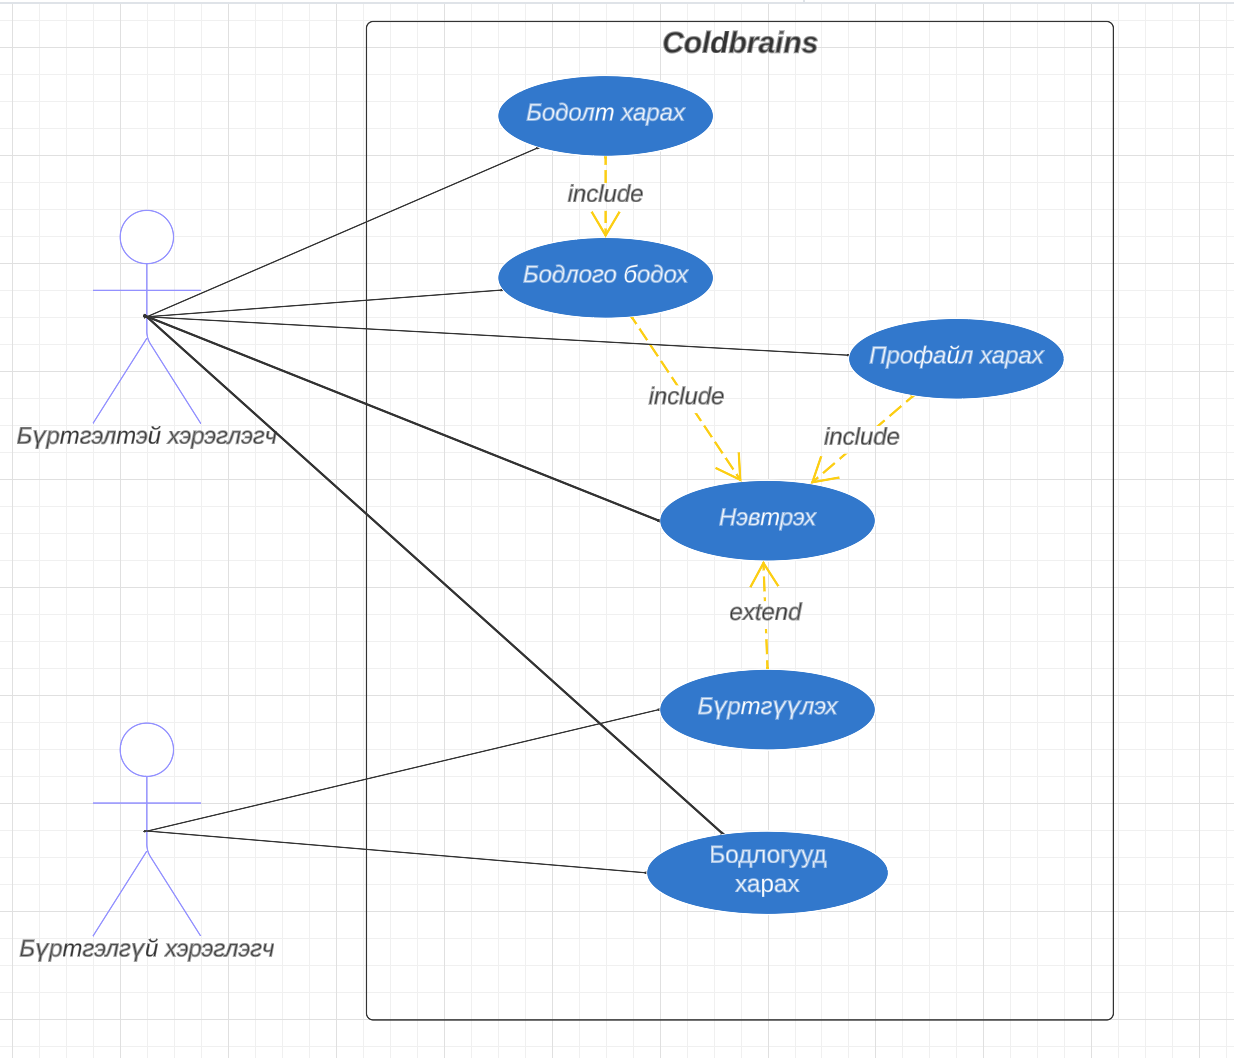
\includegraphics{img/diagrams/use-case.PNG}
  \caption{Ажлын явцын диаграм}
\end{figure}

Хэрэглэгчийг бүртгэлтэй болон бүртгэлгүй гэж ангилвал бүртгэлгүй хэрэглэгч нь системтэй танилцах зорилгоор бодлогуудын жагсаалтыг харах боломжтой бол бүртгэлтэй хэрэглэгч нь тухайн бодлогуудыг бодох, амжилттай бодсон бол бодолтуудыг харах, мөн өөрийн профайл хэсгийг харах боломжтой болно.

\clearpage